\documentclass[12pt,twoside]{article}
\usepackage{jmlda}
\newcommand{\hdir}{.}
\usepackage{hyperref}       % clickable links
\usepackage{lineno}
\usepackage{graphicx,multicol}
\usepackage{cite}
\usepackage{tikz}
\usetikzlibrary{shapes,arrows,shadows}

\bibliographystyle{jmlda_eng}
%\renewcommand{\baselinestretch}{1.4}


\newcommand{\bx}{\mathbf{x}}
\newcommand{\by}{\mathbf{y}}
\newcommand{\bw}{\mathbf{w}}
\newcommand{\bY}{\mathbf{Y}}
\newcommand{\bX}{\mathbf{X}}
\newcommand{\bu}{\mathbf{u}}
\newcommand{\bt}{\mathbf{t}}
\newcommand{\bp}{\mathbf{p}}
\newcommand{\bq}{\mathbf{q}}
\newcommand{\bg}{\mathbf{g}}
\newcommand{\bh}{\mathbf{h}}
\newcommand{\bv}{\mathbf{v}}
\newcommand{\be}{\mathbf{e}}
\newcommand{\bc}{\mathbf{c}}
\newcommand{\bP}{\mathbf{P}}
\newcommand{\bT}{\mathbf{T}}
\newcommand{\bQ}{\mathbf{Q}}
\newcommand{\bE}{\mathbf{E}}
\newcommand{\bF}{\mathbf{F}}
\newcommand{\bU}{\mathbf{U}}
\newcommand{\bI}{\mathbf{I}}
\newcommand{\bJ}{\mathbf{J}}
\newcommand{\btheta}{\boldsymbol{\theta}}
\newcommand{\bTheta}{\boldsymbol{\Theta}}



\title
	{Снижение размерности пространства зависимой переменной в задачах прогнозирования.}
\author
	{Мария Владимирова, Роман Исаченко}
\email
    {\href{mailto:vladimirova.maria@phystech.edu}{vladimirova.maria@phystech.edu}, 
    \href{mailto:isa-ro@yandex.ru}{isa-ro@yandex.ru}}
\organization
    {Московский физико-технический институт}
\abstract
	{\textcolor{blue}{В работе решается задача обнаружения зависимостей в прогнозируемой переменной. 
    Используется набор гомогенных моделей, восстанавливающих прогноз по общему для всех переменных описанию объектов. 
    Рассматривается линейная модель метода частный наименьших квадратов и ее предложенная нелинейная модификация. 
    Находятся оптимальные параметрические преобразования исходных пространств объектов и ответов. 
    Проводится вычислительный эксперимент на реальных данных объемов потребления электроэнергии и данных сигналов кортикограмм.}

    \bigskip
	\noindent
	\textbf{Ключевые слова}: \emph {прогнозирование временных рядов; мультиколлинеарность; метод частных наименьших квадратов; PLS; нелинейный PLS} 
	}

\thanks{Проект поддержан грантом РФФИ \No 16-07-01155.}


\begin{document}
\maketitle


\linenumbers
%%%%%%%%%%%%%%%%%%%%%%%%%%%%%%%%%%%%%%%%%%%%%%%%%%%%%%%%%%%%%%%%%%%%%%%%%%%%%%
\section{1. Введение}
%%%%%%%%%%%%%%%%%%%%%%%%%%%%%%%%%%%%%%%%%%%%%%%%%%%%%%%%%%%%%%%%%%%%%%%%%%%%%%

% В рассматривается рассматривается проблема проектирования Brain-Computer Interface (BCI). Мы решаем проблему выбора функций в моделях регрессии в приложении к декодированию движения на основе электрокардиограмм (ЭКГ). Задача состоит в том, чтобы предсказать траектории руки из временных рядов напряжения кортикальной активности. Описание функции каждой точки находится в пространственно-временной частотной области и включает в себя сами временные ряды напряжения и их спектральные характеристики. Выбор функции имеет решающее значение для адекватного решения проблемы регрессии, поскольку электрокортикальные данные являются высокомерными и измерения коррелируют как во временной, так и в пространственной областях.


% Система Brain-Computer Interface (BCI) улучшает умственные и физические возможности пользователя, обеспечивая прямую связь между мозгом и компьютером. BCI направлены на восстановление поврежденных функциональных возможностей пациентов с механическими или когнитивными нарушениями. Проблема проектирования BCI далеко не решается, но это обещает большой потенциал для вспомогательных технологий, реабилитационных устройств и немедицинских применений. В этой статье мы пытаемся внести вклад в разработку BCI, предложив новый метод выбора признаков в прогнозировании движения и реконструкции.
% Анализ кортикальной активности во время моторных изображений необходим для проектирования BCI. Цель анализа автомобильных изображений заключается в распознавании предполагаемых движений из зарегистрированной активности мозга. Хотя существуют различные методы измерения кортикальных данных для BCI [14, 1], мы концентрируемся на сигналах ElectroCorticoGraphic (ECoG) [10]. ECoG, а также другие инвазивные методы обеспечивают более стабильные записи и лучшее разрешение во временных и пространственных областях, чем его неинвазивные аналоги.

% Первым шагом к прогнозированию предполагаемых движений является научиться реконструировать фактические перемещения из кортикальной активности. Рассматривается проблема непрерывной реконструкции траектории. Субдуральные сигналы ECoG измеряются через 32 или 64 канала, когда субъект перемещает руку [18]. Когда сигналы ECoG трансформируются в информационные функции, проблема восстановления траектории является проблемой регрессии. Извлечение функции включает в себя применение некоторого спектрально-временного преобразования к сигналам ECoG с каждого канала [13, 15, 9]. Так как результирующее пространственно-временное спектральное представление сильно избыточно, используются различные методы выбора объектов и уменьшения размерности [17, 16], чтобы извлечь только наиболее важные функции.
% Многостороннее представление активно используется при анализе биоматериалов и химических данных благодаря многоходовой структуре данных в этих областях. Развертывание многоходовых данных в плоские матрицы может привести к пренебрежению важными зависимостями, присутствующими в развернутом измерении многопоточных данных. Напротив, многосторонние подходы сохраняют структуру данных и улучшают качество регрессии, что было продемонстрировано в [17] для регрессии частичных наименьших квадратов (PLS). Регрессия PLS и ее расширения для многопутевых данных [10, 17] доказали свою эффективность в реконструкции траектории ручной работы на ЭкоГ [17, 9, 7]. Аналогично оригинальной PLS, основанной на разложении сингулярных значений, многопоточные расширения PLS полагаются на многопоточные разложения, такие как разложение Tucker или PARAFAC [8]. Кроме того, было предложено несколько методов регуляризации для повышения его стабильности [10] и сокращения переобучения.

\textcolor{red}{В работе решается задача прогнозирования потребления электроэнегрии на основе исторических данных. 
Электрическая энергия является важной движущей силой экономического развития, а точность прогнозов спроса является важным фактором, который ведет к успешному эффективному планированию. 
По этой причине энергетическим аналитикам необходимо руководство для лучшего выбора наиболее подходящих методов прогнозирования, чтобы обеспечить точные прогнозы тенденций потребления электроэнергии.}
Для решения этой задачи используется авторегрессионная модель. Предполагается, что значение сигнала в данный момент времени линейно зависит от предыдущих значений этого же сигнала. 
Авторегрессионная модель является неустойчивой в случае наличия мультиколлинеарности в исторических данных. 
Для решения этой проблемы необходимо используются методы отбора признаков~\cite{Adolph}, в результате чего повышается устойчивость модели без существенного снижения качества прогноза.

В работе исследуются методы отбора признаков: метод частных наименьших квадратов (PLS) \cite{Ng2013} и предложенная его нелинейная модицикация (cnlPLS).
Метод частных наименьших квадратов основан на снижении размерности матрицы признаков и выделяет линейные комбинации признаков, которые оказывают наибольшее влияние на вектор ответов. 
Выделение признаков происходит итеративно, в порядке уменьшения их влияния на вектор ответов \cite{Ng2013}. Рассматриваются только значимые комбинации признаков, незначительно потеряв в точности прогноза. 

Методы PLS регрессии подробно описаны в работах~\cite{Geladi1988, Hoskuldsson1988}. 
Разницу между методом PLS и связанными с ним подходами, различные разновидности регрессии PLS можно найти в~\cite{Lehky2014}.

Нелинейное расширение метода PLS регрессии впервые введено в~\cite{Frank1990}. 
В литературе были разработаны различные модификации PLS. 
Например, функции активации искусственных нейронных сетей используются в методе PLS~\cite{Malthouse1997}. \textcolor{red}{ПОДРОБНЕЕ}
Поскольку функции активации обеспечивают нелинейные преобразования, решается проблема мультиколлинеарности. 
Предложены нелинейные методы PLS, основанные на различных моделях:  искусственных нейронных сетей~\cite{Mcavovt1992}, функции активации радиальных оснований\cite{Yan2003}, логистическая функция активации и методы оптимизации роевых частиц~\cite{Zhou2007}, используют прямые нейронные сети~\cite{Xuefeng2010}, искусственую нейронную сеть Эльмана~\cite{Bulut2014}.

Предлагается провести модификацию алгоритма PLS: совершить криволинейное и нелинейное преобразования пространства целевой переменной для учета зависимостей между сигналами в разные моменты времени.


В работе проведено сравнение двух методов отбора признаков в задаче авторегрессионного прогнозирования сигналов (PLSR и cnlPLSR). 
Цель регрессии PLS~\cite{Abdi2003}~---предсказать $\bY$ по $\bX$ и описать их общую структуру. 
Когда $\bY$~--- вектор, а $\bX$~--- матрица полного ранга, эта цель может быть выполнена с использованием обычной линейной регрессии. 
Если число предикторов велико по сравнению с числом наблюдений, то $\bX$ будет сингулярной и регрессионный подход в этом случае невозможен из-за наличия мультиколлинеарности.

В качестве практической проверки данных методов в ходе вычислительного эксперимента решается задача прогнозирования на реальных данных, содержащих объемы потребления электроэнергии в Варшаве.
Результатом применения отбора признаков является снижение размерности задачи и повышение устойчивости модели без существенной потери точности прогноза.

\textcolor{red}{ Текст про кортиграмму}
 
%%%%%%%%%%%%%%%%%%%%%%%%%%%%%%%%%%%%%%%%%%%%%%%%%%%%%%%%%%%%%%%%%%%%%%%%%%%%%%
\newpage
\section{Постановка задачи прогнозирования}
%%%%%%%%%%%%%%%%%%%%%%%%%%%%%%%%%%%%%%%%%%%%%%%%%%%%%%%%%%%%%%%%%%%%%%%%%%%%%%
Рассмотривается сигнал $\mathbf{x} = [x_t]$,  $t = 1, \dots , n$, $x_t \in \mathbb{R}$. Необходимо спрогнозировать $r$ значений сигнала или отклика:  
$\mathbf{y} = [y_t]$,  $t = 1, \dots , r$, $y_t \in \mathbb{R}$. 
Прогнозом могут являться, например, $r$ последующих значений временного ряда. 
Предполагается, что $r < n$. 


Предполагается, что сигнал обладает следующими свойствами: 

\begin{itemize}
\item значения сигнала получены через одинаковые промежутки времени, 
\item в сигнале нет пропущенных значений,
\item сигнал имеет период $\tau > r$. 
\end{itemize}
Для решения задачи прогнозирования сигнала предлагается использовать авторегрессионную модель. 
В авторегрессионной модели признаками являются предыдущие значения прогнозируемого сигнала. 
Предполагается, что значение сигнала в данный момент времени линейно зависит от предыдущих значений этого же сигнала.

\textcolor{blue}{Пусть $\mathfrak{D}= \left( \bX, \bY \right)$~--- выборка,} $\mathbf{X} = \{\bx_i\}_{i=1}^m \in \mathbb{R}^{m \times n}$~--- матрица \textcolor{blue}{объектов}, $\mathbf{Y}= \{\by_i\}_{i=1}^m \in \mathbb{R}^{m \times r}$~--- матрица ответов. 
Каждая строка $\bx_i$ матрицы $\mathbf{X}$~--– локальная история сигнала ($n$ значений сигнала, начиная с момента $i$). 
Каждая строка $\by_i$ матрицы $\mathbf{Y}$~--– локальный прогноз (например, $r$ значений сигнала, начиная с момента $n+1$). \textcolor{blue}{Матрицы $\bX$ и $\bY$ имеют следующую структуру:}
$$
\left[ \mathbf{X \, | \, Y} \right] = 
    \begin{bmatrix}
        x_1 & x_2 & \dots  & x_{n} & \vrule & y_1 & y_2 & \dots  & y_{r}\\
        x_2 & x_3 & \dots & x_{n + 1} & \vrule & y_2 & y_3 & \dots  & y_{r+1}\\
        \vdots & \vdots & \ddots & \vdots & \vrule & \vdots & \vdots & \ddots & \vdots \\
        x_{m} & x_{m+1} & \dots  & x_{m+n-1} & \vrule & y_{m} & y_{m+1} & \dots  & y_{r+m-1}
    \end{bmatrix} = 
    \begin{bmatrix}
        \bx_1 & \vrule & \by_1\\
        \bx_2 &\vrule & \by_2\\
        \vdots & \vrule &  \vdots \\
        \bx_m & \vrule & \by_m
    \end{bmatrix}.
$$


В авторегрессионной модели матрица ответов представляется в виде 
$$\mathbf{Y} = f (\mathbf{X},  \bTheta) + \epsilon ( \mathbf{X} ), $$ 
где  $f (\mathbf{X},  \bTheta) = \mathbf{X} \bTheta$~--~\textcolor{blue}{линейная} модель, $\bTheta \in \mathbb{R}^{n \times r}$~--~матрица параметров модели, а~$\epsilon(\mathbf{X})\in \mathbb{R}^{n \times r}$~--~\textcolor{blue}{матрица} регрессионных остатков.


Введем  функцию ошибки $S$ на выборке $\mathfrak{D}$:
$$S(\bTheta | \mathfrak{D}) = {\bigl\| f(\mathbf{X},  \bTheta) - \mathbf{Y} \bigr\| }_2^2 =  {\bigl\| \mathbf{X}\bTheta - \mathbf{Y} \bigr\| }_2^2.$$
\textcolor{blue}{Разобъем выборку $\mathfrak{D}$ на обучающую $\mathfrak{D}_{\mathcal{L}}$ и контрольную $\mathfrak{D}_{\mathcal{C}}$, где $\mathfrak{D}_{\mathcal{L}} \cap \mathfrak{D}_{\mathcal{C}} = \emptyset,\ \mathfrak{D}_{\mathcal{L}} \cup \mathfrak{D}_{\mathcal{C}} = \mathfrak{D}$.}
% РИСУНОК
% На рис.~\ref{regression_train_test} \textcolor{red}{ПОЧЕМУ-ТО НЕ ССЫЛКА} проиллюстрировано решение задачи линейной регрессии, где в качестве объектов выступают временные ряды, а в качестве ответов~--- вектора предсказаний. Необходимо найти аппроксимирующую функцию, отображающую пространство объектов в пространство ответов с минимальной ошибкой.


%Рассмотрим матрицу
%\centerline{\includegraphics[scale=0.2]{design.eps}}
%\begin{Large}
%$$\mathbf{X}^* = \left(
%\begin{array}{c|c}
%  \underset{1 \times n}{\mathbf{x}\mathstrut} &  \underset{1 \times r}{\mathbf{y}\mathstrut} \\ 
%  \hline
%  \underset{l \times n}{\mathbf{X}_\mathcal{L}} &  \underset{l \times r}{\mathbf{Y}_\mathcal{L}} 
% \end{array}
%\right),$$
%\end{Large}

%где $\mathfrak{D}_\mathcal{L}=   \left( \mathbf{X}_\mathcal{L}, \mathbf{Y}_\mathcal{L}\right)$ -- обучающая выборка, $\mathbf{x}$ -- исторические значение сигнала $\mathbf{s}$, $l = |\mathcal{L}|$. 
Прогноз \textcolor{blue}{отклика} сигнала на $r$ следующих значений ряда~--- это ответ модели при найденных оптимальных параметрах задачи авторегрессии: $\mathbf{y} = \mathbf{x}\bTheta^*$, где 
$$ {\bTheta}^{*} = \argmin_{\bTheta \in \mathbb{R}^{n \times r}} S(\bTheta | \mathfrak{D}_\mathcal{L}).$$
 

%Решение задачи: $$ {\mathbf{W}}^{*} = {\left( {\mathbf{X}}^{\mathsf{T}} {\mathbf{X}} \right)}^{-1} {\mathbf{X}}^{\mathsf{T}} \mathbf{Y} .$$
 %Обозначим $$\mathbf{z} =  {[x_{T-\tau+2}, x_{T-\tau+3} ,\dots ,x_{T}]}^{\mathsf{T}}. $$
% Тогда прогноз для сигнала в момент $T+1$: $$x_{T+1} = \mathbf{z^{\mathsf{T}}w}.$$
%Индуктивно, используя информацию о сигнале и уже спрогнозированные значения, с помощью авторегрессионной модели спрогнозируем значение сигнала в момент времени ${T+2}$, затем ${T+3}$ и так далее до $T+\tau$.
\textcolor{blue}{
Одним из основных препятствий эффективного применения регрессионного анализа является мультиколлинеарность. Она связана с линейной зависимостью между признаками объектов. В результате мультиколлинеарности матрица парных коэффициентов корреляции и матрица $\bX^{\T} \bX$ становятся слабообусловленными, т.е. их определители близки к нулю. Это приводит к неустойчивости оценок коэффициентов регрессии, так как в их выражения входит обратная матрица $(\bX^{\T}\bX)^{-1}$, получение которой связано с делением на определитель матрицы $\bX^{\T}\bX$. }
Значения \textcolor{blue}{сигнала} в соседние моменты времени являются зависимыми.
Таким образом, наблюдается мультиколлинеарность между признаками авторегрессионной модели прогнозирования сигнала. 
Для решения проблемы мультиколлинеарности применяются методы отбора признаков. Оптимальные параметры задачи регрессии \textcolor{blue}{$\bTheta$ настраиваются} на обучающей выборке $\mathfrak{D}_\mathcal{L}$. 
Отбор признаков происходит на контрольной выборке $\mathfrak{D}_\mathcal{C}$. 

%%%%%%%%%%%%%%%%%%%%%%%%%%%%%%%%%%%%%%%%%%%%%%%%%%%%%%%%%%%%%%%%%%%%%%%%%%%%%%
\newpage
\section{Метод частных наименьших квадратов (PLS)}
%%%%%%%%%%%%%%%%%%%%%%%%%%%%%%%%%%%%%%%%%%%%%%%%%%%%%%%%%%%%%%%%%%%%%%%%%%%%%%

Метод частных наименьших квадратов проецирует матрицу объектов $\bX$ и матрицу ответов $\bY$ в пространство меньшей размерности. В отличие от метода главных компонент, метод частных наименьших квадратов учитывает взаимосвязь между матрицами $\bX$ и $\bY$.

Матрица плана $\bX$ и матрица ответов $\bY$ проецируются на пространство меньшей размерности $l$ следующим образом:
\begin{align*}
\label{pls_x_y}
    \bX &= \bT \bP^{\T} + \bE,\\
    \bY &= \bU \bQ^{\T} + \bF,
\end{align*}
где $\bT \in \mathbb{R}^{m \times l},\ \bU \in \mathbb{R}^{m \times l}$~--- матрицы объектов и ответов в спроектированном пространстве, причём $\bT^{\T} \bT = \bI_{l}$; $\bP \in \mathbb{R}^{n \times l},\ \bQ \in \mathbb{R}^{r \times l}$~--- матрицы перехода из нового пространства в старое; $\bE\in \mathbb{R}^{m \times n},\ \bF \in \mathbb{R}^{m \times r}$~--- матрицы невязок. Размеры векторов в алгоритме можно изобразить следующим образом:

\tikzstyle{sensor_x}=[draw, line width=0.3mm, fill=blue!0, text centered, minimum height=5em, text width=3em]
\tikzstyle{sensor_t}=[draw, line width=0.3mm, fill=blue!0, text centered, minimum height=5em, text width=2em]
\tikzstyle{sensor_p}=[draw, line width=0.3mm, fill=blue!0, text centered, minimum height=2em, text width=3em]
\tikzstyle{sensor_y}=[draw, line width=0.3mm, fill=blue!0, text centered, minimum height=5em, text width=2.5em]
\tikzstyle{sensor_q}=[draw, line width=0.3mm, fill=blue!0, text centered, minimum height=2em, text width=2.5em]

\hspace{1cm}
\begin{figure}[H]
\centering
\begin{tikzpicture}
    \node (x) [sensor_x]  {$\bX$};
    \node[right of = x, node distance=3em] (x_equal) {=};
    \node[sensor_t, right of = x_equal, node distance=2.5em] (t) {$\bT$};
    \node[right of = t, node distance=2.5em] (x_times) {$\times$};
    \node[sensor_p, right of = x_times, node distance=2.8em] (p) {$\bP^{\T}$};
    \node[right of = p, node distance=2.8em] (x_sum) {+};
    \node[sensor_x, right of = x_sum, node distance=2.8em] (e) {$\bE$};
    % \node[below of = x, node distance=3.5em] (x_size) {\footnotesize{$m\times n$}};
    % \node[below of = t, node distance=3.5em] (t_size) {\footnotesize{$m\times l$}};
    % \node[below of = p, node distance=2.3em] (p_size) {\footnotesize{$l\times n$}};
    % \node[below of = e, node distance=3.5em] (e_size) {\footnotesize{$m\times n$}};

    \node[below of = x, node distance=7em] (y) [sensor_y]  {$\bY$};
    \node[below of = x_equal, node distance=7em] (y_equal) {=};
    \node[sensor_t, below of = t, node distance=7em] (u) {$\bU$};
    \node[below of = x_times, node distance=7em] (y_times) {$\times$};
    \node[sensor_q, below of = p, node distance=7em] (q) {$\bQ^{\T}$};
    \node[below of = x_sum, node distance=7em] (y_sum) {+};
    \node[sensor_y, below of = e, node distance=7em] (f) {$\bF$};
\end{tikzpicture}
\caption{Размерности векторов в алгоритме PLS}
\end{figure}




Алгоритм регрессии PLS итеративно на каждом из $l$ шагов вычисляет по одному столбцу $\bt$, $\bu$, $\bp$, $\bq$, из которых формируются матрицы $\bT$, $\bU$, $\bP$, $\bQ$ соответственно. Предполагается, что вектора новых признаков $\bt$ и $\bu$ являются линейными комбинациями столбцов матриц $\bX$ и $\bY$ соответственно.

Псевдокод метода регрессии PLS приведен в алгоритме~\ref{PLSR_pseudo}. 
Во внутреннем цикле алгоритма вычисляются вектора $\bw$ и $\bc$. 
Правила обновления векторов $\bw$, $\bc$ совпадают с итерацией Power method \textcolor{red}{\cite{Mises1929}}. 
Вектора $\bw$, $\bc$ являются собственными векторами матриц $\bX^{\T} \bY \bY^{\T} \bX$ и $\bY^{\T} \bX \bX^{\T} \bY$ соответственно.
\begin{align*}
	\bw \varpropto \bX^{\T} \underbrace{\bY \overbrace{\bY^{\T} \underbrace{\bX \bw}_{\bt}}^{\bc}}_{\bu}
\end{align*}

Обновляя вектора по данным правилам, мы максимизируем ковариацию между векторами $\bt$ и $\bu$
\begin{align*}
    \max_{\bt, \bu}  \text{cov} (\bt, \bu)^2 &= \max_{\substack{\|\bw\|=1 \\ \|\bc\| = 1}} \text{cov} \left( \bX \bw, \bY \bc \right)^2 = \max_{\substack{\|\bw\|=1 \\ \|\bc\| = 1}} \text{cov} \left(\bc^{\T}  \bY^{\T} \bX \bw \right)^2 = \\
    &= \max_{\|\bw\| = 1} \text{cov} \left\|\bY^{\T} \bX \bw \right\|^2 = \max_{\|\bw\| = 1} \bw^{\T} \bX^{\T} \bY \bY^{\T} \bX \bw = \\
    & = \lambda_{\max} \left( \bX^{\T} \bY \bY^{\T} \bX \right).
\end{align*}

После завершения внутреннего цикла вычисляются вектора $\bp$, $\bq$. Для перехода на следующий шаг необходимо вычесть из матриц $\bX$ и $\bY$ одноранговые аппроксимации.

Если ковариация между новыми признаками и ответами максимальна, то можно строить регрессионную модель в пространстве меньшей размерности с сохранением уровня точности прогноза. Параметр метода частных наименьших квадратов $l \in \mathbb{N}$ определяет размерность нового пространства. Отбор признаков осуществляется в виде замены исходных признаков на $l$ новых признаков~--- линейные комбинации исходных признаков.


Чтобы получить модель регрессии, связывающую $\bY$ и $\bX$, на каждом шаге алгоритма~\ref{PLSR_pseudo} находятся коэффициенты $\beta \in  \mathbb{R}$ такие, что $\bu \approx \bt \beta$. Найденные коэффициенты образуют вектор параметров $\boldsymbol{\beta} \in \mathbb{R}^l$. 
Подставляя вектор параметров в модель~(\ref{pls_x_y}), получаем
$$
    \bY = \bU\bQ^{\T} \approx \bT \text{diag}(\boldsymbol{\beta}) \bQ^{\T} = \bX \bP\text{diag}(\boldsymbol{\beta}) \bQ^{\T} = \bX \bTheta.
$$

\begin{center}
\begin{algorithm}[h]
\caption{Алгоритм PLSR}
    \label{PLSR_pseudo}
\begin{algorithmic}[1]
\REQUIRE $\bX, \bY, l$;
\ENSURE $\bT, \bU, \bP, \bQ$;
\STATE инициализировать $\bu := \by_1$ (вектор матрицы $\bY$)
\FOR{$i=1,\dots, l$}
  \REPEAT
    \STATE $\bw := \bX^{\T} \bu / (\bu^{\T} \bu)$
    \STATE нормировать $\bw$: $\| \bw \| = 1$
    \STATE $\mathbf{t} := \bX \bw$
    \STATE $\bc := \bY^{\T} \bt / (\bt^{\T} \bt)$
    \STATE нормировать $\bc$:  $\| \bc \| = 1$
    \STATE $\bu := \bY \bc$
  \UNTIL{$\bt$ не перестанет меняться}
  \STATE сохранить $\bt$, $\bu$, $\bc$
  \STATE $\bp := \bX^{\T}\bt/(\bt^{\T}\bt),\ \bq := \bY^{\T}\bu/(\bu^{\T}\bu)$
  \STATE регрессия ($\bu$ на $\bt$): $\beta := \bu^{\T} \bt / (\bt^{\T} \bt)$ 
  \STATE $\bX := \bX - \bt \bp^{\T}$
  \STATE $\bY := \bY - \beta\bt\bq^{\T}$ 
\ENDFOR
\end{algorithmic}
\end{algorithm}
\end{center}



% \begin{center}
% \begin{algorithm}
% \begin{algorithmic}[1]
% \REQUIRE $\mathbf{X}, \mathbf{Y}, l$;
% \ENSURE $\mathbf{T}, \mathbf{U}, \mathbf{P}, \mathbf{Q}$;
% \FOR{$i=1,\dots,l$}
%   \STATE $\mathbf{u} := \mathbf{y}_j$ для произвольного $j$
%   \REPEAT
%     \STATE $\mathbf{p := \dfrac{X^{\mathsf{T}}u}{\left\|X^{\mathsf{T}}u \right\|}}$
%     \STATE $\mathbf{t := Xp}$
%     \STATE $\mathbf{q := \dfrac{Y^{\mathsf{T}}t}{\left\|Y^{\mathsf{T}}t \right\|}} $
%     \STATE $\mathbf{u := Yq}$
%   \UNTIL{$\mathbf{t}$ не перестанет меняться}
%   \STATE сохранить $\mathbf{t}$, $\mathbf{u}$, $\mathbf{p}$, $\mathbf{q}$
%   \STATE  $\mathbf{X := X - tp^{\T}}$
%   \STATE $\mathbf{Y := Y - uq^{\T}}$
% \ENDFOR
% \end{algorithmic}
% \end{algorithm}
% \end{center}



% \begin{equation}
% \mathbf{p} = \argmax_{\left\| \mathbf{w} \right\| = 1} \text{Var}(\mathbf{Xw})  {\left( \text{Corr}\left(\mathbf{Y}, \mathbf{Xw}\right)\right)}^\mathsf{T} {\left( \text{Corr}\left(\mathbf{Y}, \mathbf{Xw}\right)\right)}
% \end{equation}

%%%%%%%%%%%%%%%%%%%%%%%%%%%%%%%%%%%%%%%%%%%%%%%%%%%%%%%%%%%%%%%%%%%%%%%%%%%%%%
\newpage
\section{Модификация метода частных наименьших квадратов (cnlPLS)}
%%%%%%%%%%%%%%%%%%%%%%%%%%%%%%%%%%%%%%%%%%%%%%%%%%%%%%%%%%%%%%%%%%%%%%%%%%%%%%
Предлагается провести модификацию алгоритма PLS: совершить криволинейное и нелинейное преобразования пространства целевой переменной  и независимой переменной для учета мультиколлинеарности между сигналами в разные моменты времени. Схема модифицированного алгоритма представлена на рис.~4. 

%FIGURE 2

% \tikzstyle{sensor_x}=[draw, fill=blue!0, text width=4em, 
%     text centered, minimum height=5em]
% \tikzstyle{sensor_y}=[draw, fill=blue!0, text width=2.7em, 
%     text centered, minimum height=5em]
% \begin{figure}[H]
% \label{scheme_cnlPLS}
% \centering
% {\footnotesize
% \def\blockdist{2.3}
% \def\edgedist{2.5}
% \vspace{1cm}
% \hspace{1cm}
% \begin{tikzpicture}
%     \node (x) [sensor_x]  {$\bX$};
%     \path (x.south)+(0,-2) node (tilde_x) [sensor_x] {$\tilde \bX$};
%     \path (x.east)+(4,0) node (y) [sensor_y] {$\bY$};
%     \path (y.south)+(0,-2) node (tilde_y) [sensor_y] {$\tilde \bY$};
%     \path (tilde_x.south)+(0,-0.8) node (x_form) {$\tilde \bX = \bT \bP^{T} + \bE$};
%     \path (tilde_y.south)+(0.4,-0.8) node (y_form) {$\tilde \bY = \bU \bQ^{\T} + \bM$};
%     \path (tilde_x.south)+(2.5,-1.3) node (u_form) {$\bU = \bT \bD + \bZ$};


%     \path [draw, ->] (x.south) -- node [right] {$f_x(\bX, \bv_x)$} 
%         (tilde_x.north);
%     \path [draw, ->] (y.south) -- node [right] {$f_y(\bY, \bv_y)$} 
%         (tilde_y.north);
%     %tilde X
%     \path [draw, -] +(1,-2) -- node [right] {$\bt$}
%       +(1,-3.7);
%     \path [draw, -] +(0.8,-3.9) -- node [below] {$\bp$}
%       +(-0.8,-3.9); 
%     %tilde Y
%     \path [draw, -] +(4.05,-2) -- node [left] {$\bu$}
%       +(4.05,-3.7);
%     \path [draw, -] +(4.2,-3.9) -- node [below] {$\bq$}
%       +(5.4,-3.9);

%     \path [draw, ->] +(0.79,-3.77) -- node [above] {$\bw$}
%       +(2.31,-4.8);
%     \path [draw, ->] +(4.21,-3.77) -- node [above] {$\bc$}
%       +(1.9,-4.8);
% \end{tikzpicture}
% }
% \caption{Схема модифицированного метода частных наименьших квадратов}
% \end{figure}

%%%%%%%%%%%%%%%%%%%%%%%%%%%%%%%%%%%%%%%%%%%%%%%%%%%%%%%%%%%%%%%%%%%%%%%%%%%%%%
\subsection{Преобразование зависимой переменной}
%%%%%%%%%%%%%%%%%%%%%%%%%%%%%%%%%%%%%%%%%%%%%%%%%%%%%%%%%%%%%%%%%%%%%%%%%%%%%%

    Рассматриваются следующие преобразования пространства зависимой переменной $\bY$:
    \begin{itemize} 
    \item криволинейное с вектором параметров $\bv$ (примеры преобразований представлены в таб.~\ref{table_functions})
    \begin{equation}
    \label{transf_y}
        \breve \bY = g (\bY, \bv),
    \end{equation}
    \item нелинейное непараметрическое преобразование
    \begin{equation*}
        \hat \bY = h (\bY),
    \end{equation*}
    \item суперпозиция преобразований   $
    \begin{diagram}
    \node{\bY}
    \arrow{e,t}{g(\bY, \bv)}
    \node{\breve \bY}
    \arrow{e,t}{h(\breve \bY)}
    \node{\tilde \bY}
    \end{diagram}
    $
    \begin{equation*}
        \tilde \bY = h (\breve \bY) = h( g( \bY, \bv)) = f(\bY, \bv).
    \end{equation*}

    \end{itemize}


    % $$
    %     \begin{diagram}
    %     \node{\bY}
    %     \arrow{e,t}{g(\bY, \bv)}
    %     \node{\breve \bY}
    %     \arrow{e,t}{h(\breve \bY)}
    %     \node{\tilde \bY}
    %     \end{diagram}
    %     $$
 
% \begin{table}
% \centering
% \begin{tabular}{l|l|l|l|}
% \cline{2-4}
%   & \textbf{Функция}                                 & \textbf{Параметры} & \textbf{Обратная}                                             \\ \cline{2-4} 
% 1 & $g(x) = \sign(x)\exp(a)(\exp(b|x|) - 1$          & $a, b > 0$         & $g^{-1}(y) = \sign(y) \exp(-b)\log(|y| \exp(-a) + 1)$         \\ \cline{2-4} 
% 2 & $g(x) = \sign(x)\exp(a)(\exp(b\ln(1+ \,|x|) - 1$ & $a, b > 0$         & $g^{-1}(y) = \sign(y)\exp( \exp(-b)\log(|y| \exp(-a) + 1)-1)$ \\ \cline{2-4} 
% 3 & $g(x) = \sign(x)\exp(a)(\exp(b|x|^{1/2}) - 1$    & $a, b > 0$         & $g^{-1}(y) = \sign(y) (\exp(-b)\log(|y| \exp(-a) + 1))^2$     \\ \cline{2-4} 
% 4 & $g(x) = \sign(x)\exp(a)(\exp(b|x|^{1/3}) - 1$    & $a, b > 0$         & $g^{-1}(y) = \sign(y) (\exp(-b)\log(|y| \exp(-a) + 1))^3$     \\ \cline{2-4} 
% 5 & $g(x) = \sign(x)\exp(a)(\exp(b|x|^{1/4}) - 1$    & $a, b > 0$         & $g^{-1}(y) = \sign(y) (\exp(-b)\log(|y| \exp(-a) + 1))^4$     \\ \cline{2-4} 
% 6 & $g(x) = \sign(x)\exp(a)(\exp(b|x|^{2}) - 1$      & $a, b > 0$         & $g^{-1}(y) = \sign(y) (\exp(-b)\log(|y| \exp(-a) + 1))^{1/2}$ \\ \cline{2-4} 
% \end{tabular}
% \caption{Криволинейные преобразования}
% \label{table_functions}
% \end{table}  
Криволинейные преобразования выбирались таким образом, чтобы функции преобразования удовлетворяли следующим условиям:
\begin{itemize}
    \item отображает множество действительных чисел во множество действительных чисел $g: \mathbb{R} \to \mathbb{R}$,
    \item принимает нулевое значение в нуле $g(0) = 0$,
    \item дифференцируется по параметрам,
    \item является обратимой, то есть существует $g^{-1}$.
\end{itemize}

\begin{table}[]
\centering
\begin{tabular}{|l|l|l|}
\hline
\textbf{№} & \textbf{Функция}                                  & \textbf{Параметры} \\ \hline
1          & $g(x) = \sign(x)\exp(a)(\exp(b|x|) - 1)$          & $a, b > 0$         \\ \hline
2          & $g(x) = \sign(x)\exp(a)(\exp(b\ln(1+ \,|x|) - 1)$ & $a, b > 0$         \\ \hline
3          & $g(x) = \sign(x)\exp(a)(\exp(b|x|^{1/2}) - 1)$    & $a, b > 0$         \\ \hline
4          & $g(x) = \sign(x)\exp(a)(\exp(b|x|^{1/3}) - 1)$    & $a, b > 0$         \\ \hline
5          & $g(x) = \sign(x)\exp(a)(\exp(b|x|^{1/4}) - 1)$    & $a, b > 0$         \\ \hline
6          & $g(x) = \sign(x)\exp(a)(\exp(b|x|^{2}) - 1)$      & $a, b > 0$         \\ \hline
\end{tabular}
\caption{Криволинейные преобразования}
\label{table_functions}
\end{table}

    Предлагается подход для обновления весов $\bv$, основаный на линеаризации функции преобразования. Разложим (\ref{transf_y}) в ряд Тейлора до второго порядка: 
    $$
        \breve \bu \approx \breve \bu_{0} + \frac{\partial \bu}{\partial \bv} \Delta \bv,
    $$
    где $\breve \bu_{0}$~--- это значение функции $g$ при известном значении переменной $\bu$.
    Для вычисления $\Delta \bv$ предложены следующие шаги. Рассматривается разница $\breve \bu - \breve \bu_{0} = \frac {\partial \bu}{\partial \bv} \Delta \bv$. Определется рассогласование $\be$
    $$
        \be = \breve \bu - \breve \bu_{0} = \frac {\partial \bu}{\partial \bv} \Delta \bv = \bJ_u \Delta \bv,
    $$
    где матрица $\bJ_u$ состоит из частных производных $\left\{\frac {\partial \bu}{\partial v_i} \right\}_{i=1}^N$, вычисленных при известном значении переменной $\bu$. Таким образом, 
    \begin{align*}
        \bJ_u &= \frac {\partial \bu}{\partial \bv} = \frac {\partial (\tilde \bY \bc)}{\partial \bv}  = \frac {\partial \left(\tilde \bY \tilde \bY^{\T}\bt \right)}{\partial \bv}  \frac1{(\bt^{\T}\bt)} = \frac {\partial \left(f (\bY, \bv) f^{\T} (\bY, \bv) \bt \right)}{\partial \bv}\frac1{(\bt^{\T}\bt)} \\
        &= \frac {\partial \left(f (\bY, \bv) \right)}{\partial \bv}  \frac{f^{\T} (\bY, \bv) \bt }{(\bt^{\T}\bt)} + f (\bY, \bv) \frac {\partial \left(f^{\T} (\bY, \bv) \bt \right)}{\partial \bv} \frac1{(\bt^{\T}\bt)}.
    \end{align*}

    Далее $\Delta \bv$ вычисляется решением задачи регрессии рассогласования $\be$ так, что 
  \begin{equation}
  \label{delta_v}
    \Delta \bv  = (\bJ_u^{\T} \bJ_u)^{-1} \bJ_u^{\T} \be.
  \end{equation}

  %%%%%%%%%%%%%%%%%%%%%%%%%%%%%%%%%%%%%%%%%%%%%%%%%%%%%%%%%%%%%%%%%%%%%%%%%%%%%%
\subsection{Преобразование независимой переменной}
%%%%%%%%%%%%%%%%%%%%%%%%%%%%%%%%%%%%%%%%%%%%%%%%%%%%%%%%%%%%%%%%%%%%%%%%%%%%%%
    Аналогично преобразованию целевой переменной $\bY$, совершается преобразование зависимой переменной $\bX$ для учета мультиколлинеарности в признаковом пространстве. 

    Рассмотрим преобразования $\bX$
    \begin{itemize} 
    \item криволинейное с вектором параметров $\bv$ (таб.~\ref{table_functions})
    \begin{equation}
    \label{transf_y}
        \breve \bX = g (\bX, \bv_x),
    \end{equation}
    \item нелинейное непараметрическое преобразование
    \begin{equation*}
        \hat \bX = h (\bX),
    \end{equation*}
    \item суперпозиция преобразований 
    \begin{equation*}
        \tilde \bX = h (\breve \bX) = h( g( \bX, \bv_x)) = f(\bX, \bv_x).
    \end{equation*}
    \end{itemize}

%%%%%%%%%%%%%%%%%%%%%%%%%%%%%%%%%%%%%%%%%%%%%%%%%%%%%%%%%%%%%%%%%%%%%%%%%%%%%%
\subsection{Алгоритм cnlPLSR}
%%%%%%%%%%%%%%%%%%%%%%%%%%%%%%%%%%%%%%%%%%%%%%%%%%%%%%%%%%%%%%%%%%%%%%%%%%%%%%
    В данном разделе представлен модифицированный метод PLSR, содержащий шаги преобразования целевой переменной. Аналогично методу PLSR (алгоритм~\ref{PLSR_pseudo}), алгоритм \ref{cnlPLSR_pseudo} начинается с инициализации вектора $\bu$, а обновления весов преобразования считается с помощью рассогласования $\be$ для вектора $\bu$, вычисленного в цикле и на предыдущей итерации.
    \vspace{-0.5cm}
\begin{center}
\begin{algorithm}[H]
\caption{Алгоритм cnlPLSR с преобразованием пространства ответов}
    \label{cnlPLSR_pseudo}
\begin{algorithmic}[1]
\REQUIRE $\bX, \bY, l$;
\ENSURE $\bT, \bU, \bP, \bQ$;
\STATE инициализировать $\bv$
\STATE определить $\bu_0$ как вектор преобразования $f(\bY, \bv)$
\FOR{$i=1,\dots, l$}
  \REPEAT
    \STATE $\bw := \bX^{\T} \bu_0 / (\bu_0^{\T} \bu_0)$
    \STATE нормировать $\bw$: $\| \bw \| = 1$
    \STATE $\bt := \bX \bw$
    \STATE $\tilde \bY = f(\bY, \bv)$
    \STATE $\bc := \tilde \bY^{\T} \bt / (\bt^{\T} \bt)$
    \STATE нормировать $\bc$: $\| \bc \| = 1$
    \STATE $\bu := \tilde \bY \bc$
    \STATE $\be := \bu - \bu_0$
    \STATE $\bJ := \partial \bu / \partial \bv$
    \STATE $\Delta \bv = (\bJ^{\T} \bJ)^{-1} \bJ^{\T} \be$
    \STATE $\bv := \bv + \Delta \bv,\ \|\bv\| = 1$
    \STATE $\bu_0 := \bu$
  \UNTIL{$\bt$ не перестанет меняться}
  \STATE сохранить $\bt$, $\bu$, $\bc$
  \STATE вычислить $\tilde \bY$
  \STATE $\bp := \bX^{\T}\bt/(\bt^{\T}\bt),\ \bq := \tilde \bY^{\T}\bu/(\bu^{\T}\bu)$
  \STATE регрессия ($\bu$ на $\bt$): $\beta := \bu^{\T} \bt / (\bt^{\T} \bt)$ 
  \STATE $\bX := \bX - \bt\bt^{\T}\bX/(\bt^{\T}\bt)$
  \STATE $\tilde{\bY} := \tilde \bY - \beta\bt\bc^{\T}$
  \STATE вычислить $\bY$ с помощью обратного преобразования $f^{-1}(\tilde \bY, \bv)$
\ENDFOR
\end{algorithmic}
\end{algorithm}
\end{center}

\begin{center}
\begin{algorithm}[H]
\caption{Алгоритм cnlPLSR с преобразованием пространства объектов}
    \label{cnlPLSR_pseudo_x}
\begin{algorithmic}[1]
\REQUIRE $\bX, \bY, l$;
\ENSURE $\bT, \bU, \bP, \bQ$;
\STATE инициализировать $\bv_x$
\STATE определить $\bt_0$ \textcolor{red}{КАК}
\STATE определить $\bu$ как вектор матрицы $\bY$
\FOR{$i=1,\dots, l$}
  \REPEAT
    \STATE $\tilde \bX := f(\bX, \bv_x)$
    \STATE $\bw := \tilde \bX^{\T} \bu / (\bu^{\T} \bu)$
    \STATE нормировать $\bw$: $\| \bw \| = 1$
    \STATE $\bt := \tilde \bX \bw$
    \STATE $\bc := \bY^{\T} \bt / (\bt^{\T} \bt)$
    \STATE нормировать $\bc$: $\| \bc \| = 1$
    \STATE $\bu := \bY \bc$
    \STATE \textcolor{red}{?} $\be := \bt - \bt_0$
    \STATE \textcolor{red}{?} $\bJ_t := \partial \bt / \partial \bv_x$
    \STATE \textcolor{red}{?} $\Delta \bv_x = (\bJ_t^{\T} \bJ_t)^{-1} \bJ_t^{\T} \be$
    \STATE $\bv_x := \bv_x + \Delta \bv_x,\ \|\bv_x\| = 1$
    \STATE \textcolor{red}{?} $\bt_0 := \bt$
  \UNTIL{$\bt$ не перестанет меняться}
  \STATE сохранить $\bt$, $\bu$, $\bc$
  \STATE вычислить $\tilde \bY$
  \STATE $\bp := \bX^{\T}\bt/(\bt^{\T}\bt),\ \bq := \tilde \bY^{\T}\bu/(\bu^{\T}\bu)$
  \STATE регрессия ($\bu$ на $\bt$): $\beta := \bu^{\T} \bt / (\bt^{\T} \bt)$ 
  \STATE $\bX := \bX - \bt\bt^{\T}\bX/(\bt^{\T}\bt)$
  \STATE $\tilde{\bY} := \tilde \bY - \beta\bt\bc^{\T}$
  \STATE вычислить $\bY$ с помощью обратного преобразования $f^{-1}(\tilde \bY, \bv)$
\ENDFOR
\end{algorithmic}
\end{algorithm}
\end{center}

%%%%%%%%%%%%%%%%%%%%%%%%%%%%%%%%%%%%%%%%%%%%%%%%%%%%%%%%%%%%%%%%%%%%%%%%%%%%%%
\newpage
\section{Вычислительный эксперимент}
%%%%%%%%%%%%%%%%%%%%%%%%%%%%%%%%%%%%%%%%%%%%%%%%%%%%%%%%%%%%%%%%%%%%%%%%%%%%%%
В рамках вычислительного эксперимента строится прогноз временных рядов. В ходе эксперимента сравниваются методы PLSR, нелинейных автоэнкодеров и cnlPLS. Сравнение проводится на реальных данных объемов потребления электроэнергии в Польше. 

Вычислительный эксперимент, продемонстрированный в этом разделе, основан на данных электроэнергии. Данные состоят из временного ряда польских электрических нагрузок и временных рядов погоды в Варшаве (долгота: 21,25, широта: 52,30, высота над уровнем моря: 94). Временные ряды энергии состоят из почасовых записей (всего 52512 наблюдений), а погодные измерения проводились раз в день и содержат 2188 наблюдений. Многомасштабные временные ряды соответствуют периоду 1999-2004 годов. Результаты, полученные с этим набором данных, являются иллюстрацией предлагаемых методов, поскольку данные содержат многомасштабне временные ряды, имеющие различный характер.

Примеры работы алгоритма приведены на рис.~\ref{fig:forecast}. Метод успешно делает краткосрочный прогноз (до 10 дней). С увеличением горизонта прогнозирования предсказание смещается. 


% Require \usepackage{subfig}

% \begin{figure}[H]
%     \centering
%     \begin{subfigure}[b]{0.3\textwidth}
%         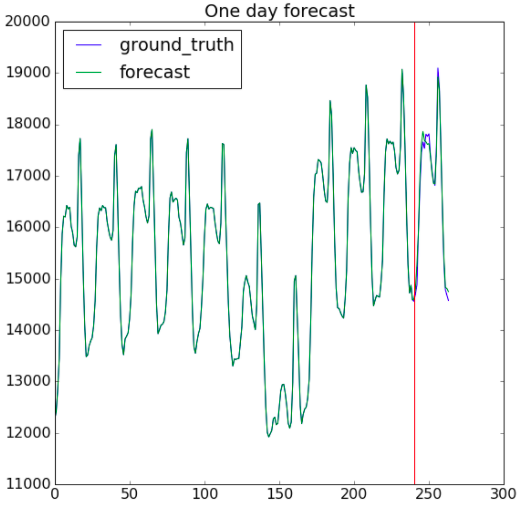
\includegraphics[width=\textwidth]{oneday.png}
%     \end{subfigure}
%     \begin{subfigure}[b]{0.3\textwidth}
%         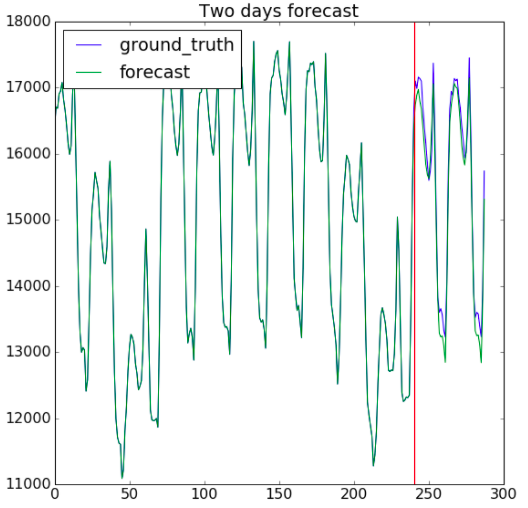
\includegraphics[width=\textwidth]{twodays.png}
%     \end{subfigure}
%     \begin{subfigure}[b]{0.3\textwidth}
%         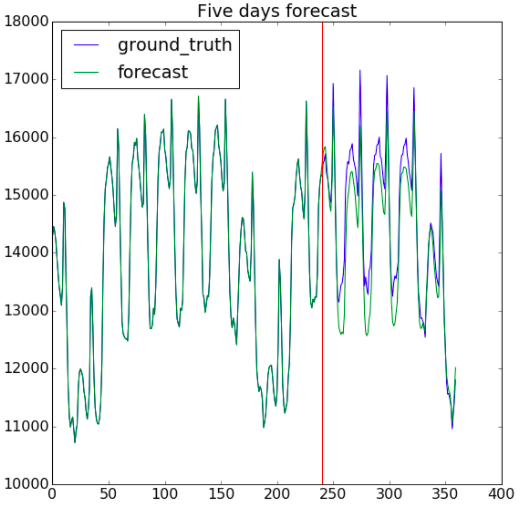
\includegraphics[width=\textwidth]{fivedays.png}
%     \end{subfigure}
%     \begin{subfigure}[b]{0.3\textwidth}
%         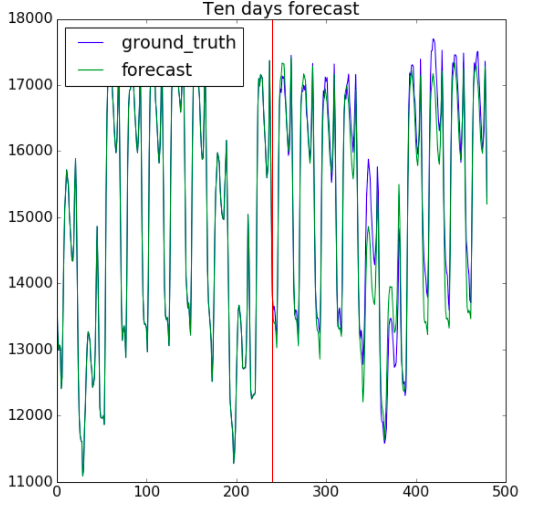
\includegraphics[width=\textwidth]{tendays.png}
%     \end{subfigure}
%     \begin{subfigure}[b]{0.3\textwidth}
%         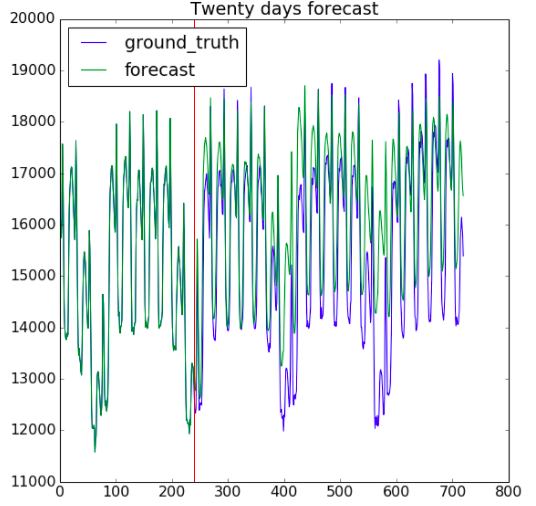
\includegraphics[width=\textwidth]{twentydays.png}
%     \end{subfigure}
%     \begin{subfigure}[b]{0.3\textwidth}
%         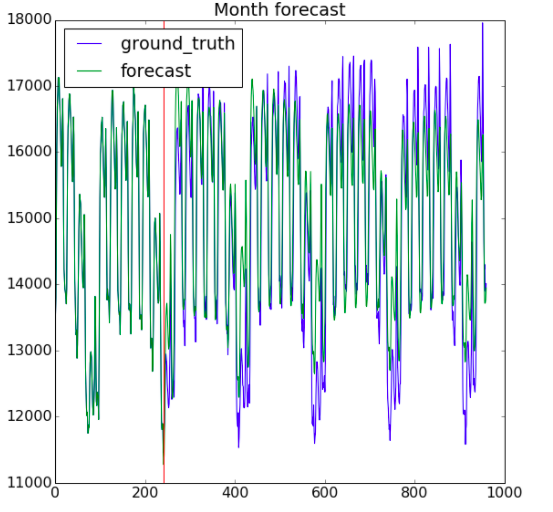
\includegraphics[width=\textwidth]{month.png}
%     \end{subfigure}
%     \caption{Прогнозирование базового алгоритма на 1, 2, 5, 10, 20, 30 дней}
%     \label{fig:forecast}
% \end{figure}

Результаты вычислительного эксперимента для предложенного модифицированного алгоритма cnlPLS представлены на рис.~\ref{fig:animals}. На графиках изображены сглаженные зависимости ошибки MSE от числа компонент в алгоритме для разных функций. Из графиков видно, что для функций $(a)-(e)$ ошибка при увеличении числа компонент падает, затем колеблется, слабо меняясь. Ошибка алгоритма с функцией $(f)$ увеличивается при увеличении числа компонент. Это означает, что преобразование, выполненное в пространстве целевой переменной с помощью функции $(f)$, плохо описывает зависимость. Меньшую ошибку имеют функции, растущие медленнее, а именно $(d)$ и $(e)$. 


% Require \usepackage{subfig}

% \begin{figure}
%     \centering
%     \begin{subfigure}[b]{0.4\textwidth}
%         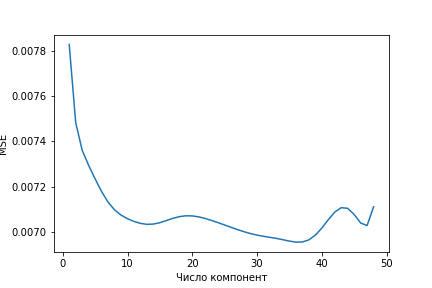
\includegraphics[width=\textwidth]{exp_abs_x.png}
%         \caption{$g(x) = \sign(x) e^a(\exp(b|x|) - 1)$}
%         \label{fig:exp_abs_x}
%     \end{subfigure}
%     ~ %add desired spacing between images, e. g. ~, \quad, \qquad, \hfill etc. 
%       %(or a blank line to force the subfigure onto a new line)
%     \begin{subfigure}[b]{0.4\textwidth}
%         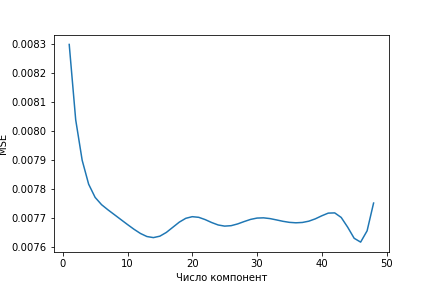
\includegraphics[width=\textwidth]{exp_log_x.png}
%         \caption{$g(x) = \sign(x)e^a(\exp(b\ln(1+ \,|x|) - 1)$}
%         \label{fig:exp_log_x}
%     \end{subfigure}
%     ~ %add desired spacing between images, e. g. ~, \quad, \qquad, \hfill etc. 
%     %(or a blank line to force the subfigure onto a new line)
%     \begin{subfigure}[b]{0.4\textwidth}
%         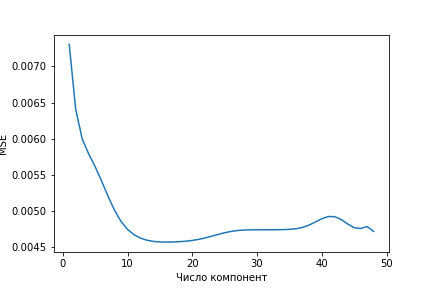
\includegraphics[width=\textwidth]{exp_x_1_2.png}
%         \caption{$g(x) = \sign(x)e^a(\exp(b|x|^{1/2}) - 1)$}
%         \label{fig:exp_x_1_2}
%     \end{subfigure}
%     \begin{subfigure}[b]{0.4\textwidth}
%         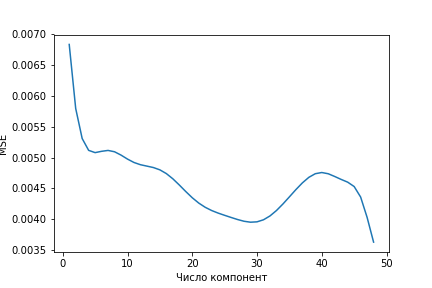
\includegraphics[width=\textwidth]{exp_x_1_3.png}
%         \caption{$g(x) = \sign(x)e^a(\exp(b|x|^{1/3}) - 1)$ }
%         \label{fig:exp_x_1_3}
%     \end{subfigure}
%     ~ %add desired spacing between images, e. g. ~, \quad, \qquad, \hfill etc. 
%       %(or a blank line to force the subfigure onto a new line)
%     \begin{subfigure}[b]{0.4\textwidth}
%         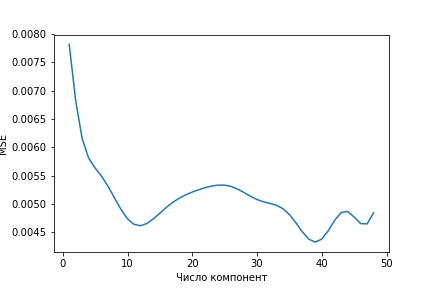
\includegraphics[width=\textwidth]{exp_x_1_4.png}
%         \caption{$g(x) = \sign(x)e^a(\exp(b|x|^{1/4}) - 1)$}
%         \label{fig:exp_x_1_4}
%     \end{subfigure}
%     ~ %add desired spacing between images, e. g. ~, \quad, \qquad, \hfill etc. 
%     %(or a blank line to force the subfigure onto a new line)
%     \begin{subfigure}[b]{0.4\textwidth}
%         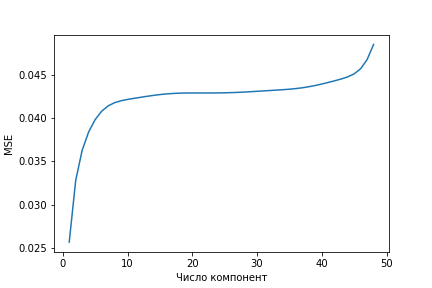
\includegraphics[width=\textwidth]{exp_x_2.png}
%         \caption{$g(x) = \sign(x)e^a(\exp(b|x|^{2}) - 1)$}
%         \label{fig:exp_x_2}
%     \end{subfigure}
%     \caption{Зависимость ошибки от числа компонент в алгоритме cnlPLS для разных функций}\label{fig:animals}
% \end{figure}

В табл.~\ref{results} продемонстрировано увеличение точности прогнозивания при использовании криволинейного преобразования в пространстве зависимой переменной, но увеличение точности в пределах погрешности алгоритма (0.0005-0.0010). Функции с быстрым ростом не позволяют описать зависимость.
\begin{table}[]
\centering
\begin{tabular}{|l|l|l|l|l|}
\hline
\textbf{Алгоритм}                                                                                  & \textbf{N=3}     & \textbf{N=5}     & \textbf{N=10}    & \textbf{N=20}    \\ \hline
PLS                                                                                                & 0,00404          & 0,00337          & \textbf{0,00151} & 0,00135          \\ \hline
\begin{tabular}[c]{@{}l@{}}cnlPLS\\ $g(x) = \sign(x)\exp(a)(\exp(b|x|) - 1)$\end{tabular}          & 0.00529          & 0.00514          & 0.00536          & 0.00506          \\ \hline
\begin{tabular}[c]{@{}l@{}}cnlPLS\\ $g(x) = \sign(x)\exp(a)(\exp(b\ln(1+ \,|x|) - 1)$\end{tabular} & 0.00362          & 0.00386          & 0.00326          & 0.00317          \\ \hline
\begin{tabular}[c]{@{}l@{}}cnlPLS\\ $g(x) = \sign(x)\exp(a)(\exp(b|x|^{1/2}) - 1)$\end{tabular}    & 0.00272          & 0.00236          & 0.00287          & \textbf{0.00128} \\ \hline
\begin{tabular}[c]{@{}l@{}}cnlPLS\\ $g(x) = \sign(x)\exp(a)(\exp(b|x|^{1/3}) - 1)$\end{tabular}    & \textbf{0.00241} & \textbf{0.00233} & 0.00221          & 0.00173          \\ \hline
\begin{tabular}[c]{@{}l@{}}cnlPLS\\ $g(x) = \sign(x)\exp(a)(\exp(b|x|^{1/4}) - 1)$\end{tabular}    & 0.00796          & 0.00768          & 0.00737          & 0.00803          \\ \hline
\begin{tabular}[c]{@{}l@{}}cnlPLS\\ $g(x) = \sign(x)\exp(a)(\exp(b|x|^{2}) - 1)$\end{tabular}      & 0.00816          & 0.00798          & 0.00796          & 0.00775          \\ \hline
\end{tabular}
\caption{Значения ошибки MSE для разных чисел компонент и разных функций}
\label{results}
\end{table}

%%%%%%%%%%%%%%%%%%%%%%%%%%%%%%%%%%%%%%%%%%%%%%%%%%%%%%%%%%%%%%%%%%%%%%%%%%%%%%
\section{Заключение}
В данной работе предложен новый подход к обнаружению зависимостей в пространстве зависимой переменной задачи прогнозирования временных рядов. Сравнивались результаты прогнозирования временных рядов, полученных с помощью метода частных наименьших квадратов и предложенной модификации. Проведен вычислительный эксперимент на реальных данных потребления электроэнергии в Варшаве. Построенная прогностическая модель показала высокое качество предсказания электрической нагрузки. 
%%%%%%%%%%%%%%%%%%%%%%%%%%%%%%%%%%%%%%%%%%%%%%%%%%%%%%%%%%%%%%%%%%%%%%%%%%%%%%
%\section*{СПИСОК ЛИТЕРАТУРЫ}

\newpage
\nocite{*}

\bibliographystyle{unsrt}
\begin{thebibliography}{10}
\def\selectlanguageifdefined#1{
\expandafter\ifx\csname date#1\endcsname\relax
\else\selectlanguage{#1}\fi}

\bibitem{thrun2012}
\BibAuthor{Thrun, Sebastian and Pratt, Lorien}
{Learning to learn}~//
Springer Science \& Business Media, 2012.

\bibitem{Chong2005} %1
%\selectlanguageifdefined{english}
\BibAuthor{Chong, Il Gyo and Jun, Chi Hyuck}
{Performance of some variable selection methods when multicollinearity is present}~//
Chemometrics and Intelligent Laboratory Systems, 2005.
Vol.~78.
No.~1.
P.~103--112.

\bibitem{Xuefeng2010} %1
%\selectlanguageifdefined{english}
\BibAuthor{Xuefeng, Yan}
{Hybrid artificial neural network based on BP-PLSR and its application in development of soft sensors}~//
Chemometrics and Intelligent Laboratory Systems, 2010.
Vol.~103.
No.~2.
P.~152--159.

\bibitem{Mcavovt1992} %1
%\selectlanguageifdefined{english}
\BibAuthor{Mcavovt, J. and Process, Chemical}
{Title }~//
Journal name, 2005.
Vol.~16.
No.~4.
P.~379--391.

\bibitem{Yan2003} %1
%\selectlanguageifdefined{english}
\BibAuthor{Yan, Xuefeng F. and Chen, Dezhao Z. and Hu, Shangxu X.}
{Chaos-genetic algorithms for optimizing the operating conditions based on RBF-PLS model}~//
Computers and Chemical Engineering, 2003.
Vol.~27.
No.~10.
P.~1393--1404.

\bibitem{Frank1990} %1
%\selectlanguageifdefined{english}
\BibAuthor{Frank, Ildiko E.}
{A nonlinear PLS model}~//
Chemometrics and Intelligent Laboratory Systems, 1990.
Vol.~8.
No.~2.
P.~109--119.

\bibitem{Zhou2007} %1
%\selectlanguageifdefined{english}
\BibAuthor{Zhou, Yan Ping and Jiang, Jian Hui and Lin, Wei Qi and Xu, Lu and Wu, Hai Long and Shen, Guo Li and Yu, Ru Qin}
{Artificial neural network-based transformation for nonlinear partial least-square regression with application to QSAR studies}~//
Talanta, 2007.
Vol.~71.
No.~2.
P.~848--853.


\bibitem{Geladi1988} %1
%\selectlanguageifdefined{english}
\BibAuthor{Chong, Il Gyo and Jun, Chi Hyuck}
{Notes on the history and nature of partial least squares (PLS) modelling}~//
Journal of Chemometrics, 1988.
Vol.~2.
No.~January.
P.~231--246.


\bibitem{Hoskuldsson1988} %1
%\selectlanguageifdefined{english}
\BibAuthor{H{\"{o}}skuldsson, Agnar}
{PLS regression}~//
Chemometrics and Intelligent Laboratory Systems, 1987.
Vol.~2.
No.~August.
P.~581--591.


\bibitem{Bulut2014} %1
%\selectlanguageifdefined{english}
\BibAuthor{Bulut, Elif and Egrioglu, Erol}
{A New Partial Least Square Method Based on Elman Neural Network}~//
Chemometrics and Intelligent Laboratory Systems, 2005.
Vol.~4.
No.~4.
P.~154--158.


\bibitem{Ng2013} %1
%\selectlanguageifdefined{english}
\BibAuthor{Ng, Kee Siong}
{A Simple Explanation of Partial Least Squares}~//
Journal title, 2013.
Vol.~volume.
No.~number.
P.~1--10.


\bibitem{Rosipal2011} %1
%\selectlanguageifdefined{english}
\BibAuthor{Rosipal, Roman}
{Nonlinear partial least squares: An overview}~//
Chemoinformatics and Advanced Machine Learning Perspectives: Complex Computational Methods and Collaborative Techniques, 2011.
Vol.~number.
No.~number.
P.~169--189.


\bibitem{Wold1989} %1
%\selectlanguageifdefined{english}
\BibAuthor{Wold, Svante and Kettaneh-Wold, Nouna and Skagerberg, Bert}
{Nonlinear PLS modeling}~//
Chemometrics and Intelligent Laboratory Systems, 1989.
Vol.~7.
No.~1-2.
P.~53--65.

\bibitem{Rosipal2006} %1
%\selectlanguageifdefined{english}
\BibAuthor{Rosipal, Roman and Kramer, Nicole}
{Overview and Recent Advances in Partial Least Squares}~//
????? C. Saunders et al. (Eds.): SLSFS 2005, LNCS 3940, 2006.
Vol.~?.
No.~?.
P.~34--51.

\bibitem{Lu2004} %1
%\selectlanguageifdefined{english}
\BibAuthor{Lu, Wen-Cong and Chen, Nian-Yi and Li, Guo-Zheng and Yang, Jie}
{Multitask Learning Using Partial Least Squares Method}~//
Proceedings of the Seventh International Conference on Information Fusion; International Society of Information Fusion, 2004.
Vol.~1.
P.~79--84.

\bibitem{Varnek2012} %1
%\selectlanguageifdefined{english}
\BibAuthor{Varnek, Alexandre and Baskin, Igor}
{Machine learning methods for property prediction in chemoinformatics: Quo Vadis?}~//
Journal of Chemical Information and Modeling, 2012.
Vol.~52.
No.~6.
P.~1413--1437.

\bibitem{Lehky2014} %1
%\selectlanguageifdefined{english}
\BibAuthor{Lehky, Sidney R. and Kiani, Roozbeh and Esteky, Hossein and Tanaka, Keiji}
{Dimensionality of object representations in monkey inferotemporal cortex}~//
Neural computation, 2014.
Vol.~1872.
No.~10.
P.~1840--1872.

\bibitem{Abdi2003} %1
%\selectlanguageifdefined{english}
\BibAuthor{Abdi, Herv{\'{e}}}
{Partial Least Squares (PLS) Regression}~//
Encyclopedia for research methods for the social sciences, 2003.
P.~792--795.

\bibitem{Caruana2003} %1
%\selectlanguageifdefined{english}
\BibAuthor{Caruana, Rich and de Sa, Virginia R.}
{Benefitting from the Variables that Variable Selection Discards}~//
Journal of Machine Learning Research, 2003.
Vol.~3.
No.~7-8.
P.~1245--1264.

\bibitem{Mises1929} %1
%\selectlanguageifdefined{english}
\BibAuthor{Mises R. V., Pollaczek‐Geiringer H. }
{Praktische Verfahren der Gleichungsauflösung}~//
ZAMM‐Journal of Applied Mathematics and Mechanics/Zeitschrift für Angewandte Mathematik und Mechanik, 1929.
Vol.~9.
No.~1.
P.~58--77.

\end{thebibliography}

\end{document}